
\section{Results}


\begin{table}[ht]
\caption{Test results of 5 classes from java package. Each class is tested 10 times by both random and DSSR strategy.fs} % title of Table
\centering % used for centering table
\begin{tabular}{| c | c | c | c | c | c | c | c | c | c | c |} % centered columns (4 columns)
\hline\hline %inserts double horizontal lines
 \begin{sideways} Serial Number \end{sideways} &  \begin{sideways} y.t.Faulty1 by Random \end{sideways} &  \begin{sideways} y.t.Faulty1 by DSSR \end{sideways} &  \begin{sideways} y.t.Faulty2 by Random \end{sideways} &  \begin{sideways} y.t.Faulty2 by DSSR \end{sideways} & \begin{sideways} y.t.Faulty3 by Random \end{sideways} &  \begin{sideways}y.t.Faulty3 by DSSR \end{sideways} &  \begin{sideways}y.t.Faulty4 by Random \end{sideways} &  \begin{sideways} y.t.Faulty4 by DSSR \end{sideways} &  \begin{sideways} y.t.Faulty5 by Random \end{sideways} &  \begin{sideways} y.t.Faulty5 by DSSR \end{sideways} \\ [1ex] % inserts table
%heading
\hline  % inserts single horizontal line
1 & 1 & 2 & 0 & 2 & 2 & 3 & 0 & 2 & 1 & 3 \\  % inserting body of 

2 & 1 & 2 & 0 & 2 & 1 & 3 & 1 & 2 & 1 & 3 \\

3 & 0 & 2 & 0 & 2 & 2 & 2 & 0 & 2 & 0 & 3 \\

4 & 1 & 2 & 0 & 2 & 1 & 2 & 1 & 2 & 1 & 2 \\

5 & 0 & 2 & 0 & 2 & 2 & 3 & 1 & 2 & 1 & 2 \\

6 & 0 & 2 & 0 & 2 & 2 & 3 & 1 & 2 & 1 & 2 \\

7 & 1 & 2 & 0 & 2 & 1 & 3 & 0 & 2 & 1 & 3 \\

8 & 1 & 1 & 0 & 2 & 1 & 3 & 1 & 1 & 2 & 3 \\

9 & 1 & 2 & 0 & 2 & 1 & 3 & 1 & 2 & 1 & 3 \\

10 & 1 & 2 & 0 & 2 & 2 & 3 & 1 & 2 & 1 & 3 \\  [1ex] % [1ex] adds vertical spacefs

\hline %inserts single line
\end{tabular}
\label{table:five} % is used to refer this table in the text
\end{table}


Experimental finding indicate that DSSR strategy performs up to 30 \% better than pure random strategy. In some cases pure random strategy is not able to find even a single fault where as DSSR strategy finds all the available faults in the given SUT. Results of the group 1 tests are given in Table \ref{table:five} and the same data is also represented by a box-plot graph given in Figure \ref{fig:Result1}.\\


After confirmation of the effectiveness of DSSR strategy from group 1 experiments we performed similar tests on 10 random classes from Java JDK in group 2. Results were not very different and DSSR strategy gave better performance as presented in Table \ref{table:tena} and \ref{table:tenb}.  The data is also represented in Figure \ref{fig:Result2} using box-plot graph.\\



\begin{figure}[htp]
\centering
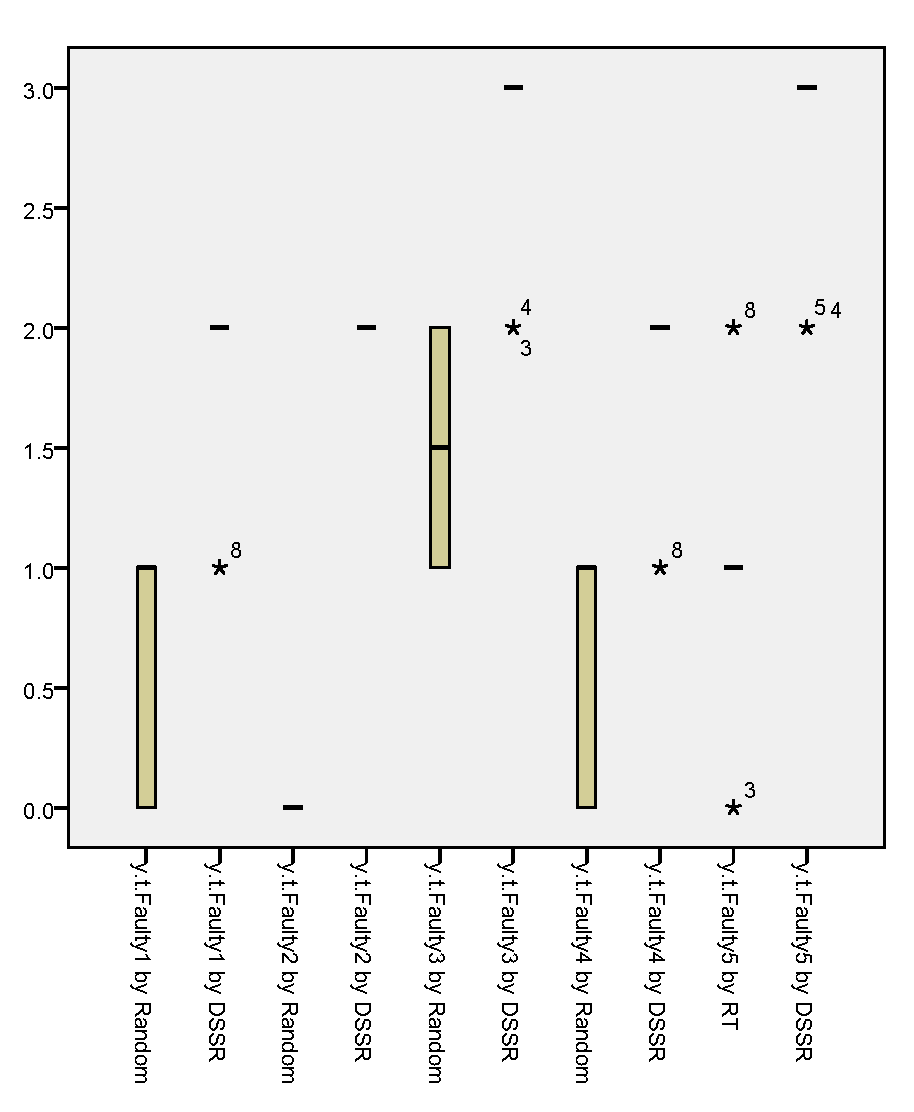
\includegraphics[width=7.5cm,height=9.5cm]{figures/owntests.png}
\caption{Test Results of 5 classes developed specially for DSSR analysis.}
\label{fig:Result1}
\end{figure}





\begin{table}[ht]
\caption{Test results of 10 classes from java package. Each class is tested 10 times by both random and DSSR strategy.fs} % title of Table
\centering % used for centering table
\begin{tabular}{| c | c | c | c | c | c | c | c | c | c | c |} % centered columns (4 columns)
\hline\hline %inserts double horizontal lines
 \begin{sideways} Serial Number \end{sideways} &  \begin{sideways} j.u.Character by Random \end{sideways} &  \begin{sideways} j.u.Character by DSSR \end{sideways} &  \begin{sideways} j.l.String by Random \end{sideways} &  \begin{sideways} j.l.String by DSSR \end{sideways} & \begin{sideways} j.u.Calendar by Random \end{sideways} &  \begin{sideways}j.u.Calender by DSSR \end{sideways} &  \begin{sideways}j.u.Scanner by Random \end{sideways} &  \begin{sideways} j.u.Scanner by DSSR \end{sideways} &  \begin{sideways} j.u.Properties by Random \end{sideways} &  \begin{sideways} j.u.Properties by DSSR \end{sideways}  \\ [0.5ex] % inserts table
%heading
\hline % inserts single horizontal line
1 & 11 & 13 & 8 & 8 & 4 & 4 & 41 & 41 & 13 & 14\\ % inserting body of 

2 & 13 & 12 & 8 & 8 & 3 & 3 & 39 & 42 & 12 & 13\\

3 & 12 & 14 & 6 & 7 & 3 & 4 & 41 & 41 & 12 & 13\\

4 & 12 & 12 & 7 & 8 & 4 & 4 & 39 & 43 & 12 & 13\\

5 & 11 & 12 & 8 & 7 & 4 & 4 & 38 & 42 & 13 & 13\\

6 & 13 & 11 & 6 & 7 & 3 & 4 & 38 & 39 & 12 & 14\\

7 & 11 & 12 & 7 & 8 & 4 & 4 & 39 & 39 & 12 & 14\\

8 & 13 & 12 & 7 & 8 & 4 & 4 & 41 & 42 & 13 & 13\\

9 & 12 & 12 & 8 & 8 & 4 & 4 & 37 & 42 & 13 & 13\\ 

10 & 13 & 14 & 4 & 7 & 4 & 4 & 40 & 41 & 14 & 13\\ [1ex] % [1ex] adds vertical spacefs

\hline %inserts single line

\end{tabular}
\label{table:tena} % is used to refer this table in the text
\end{table}


\begin{table}[ht]
\caption{Test results of 10 classes from java package. Each class is tested 10 times by both random and DSSR strategy.} % title of Table
\centering % used for centering table

\begin{tabular}{| c | c | c | c | c | c | c | c | c | c | c |} % centered columns (4 columns)
\hline\hline %inserts double horizontal lines
 \begin{sideways} Serial Number \end{sideways} & \begin{sideways} j.l.Thread by Random \end{sideways} &  \begin{sideways} j.l.Thread by DSSR \end{sideways} &  \begin{sideways} j.l.ProcessBuilder by Random \end{sideways} &  \begin{sideways} j.l.ProcessBuilder by DSSR \end{sideways} &  \begin{sideways} j.l.Double by Random \end{sideways} & \begin{sideways} j.l.Double by DSSR \end{sideways} &  \begin{sideways} j.l.ClassLoader by Random \end{sideways} &  \begin{sideways} j.l.ClassLoader by DSSR \end{sideways} & \begin{sideways} j.l.Character by Random \end{sideways} & \begin{sideways} j.l.Character by DSSR \end{sideways} \\ [0.5ex] % inserts table
%heading
\hline % inserts single horizontal line
1 & 4 & 4 & 29 & 28 & 9 & 9 & 17 & 18 & 25 & 34\\ % inserting body of 

2 & 4 & 4 & 30 & 25 & 10 & 8 & 26 & 27 & 24 & 35\\

3 & 4 & 4 & 30 & 31 & 7 & 17 & 26 & 29 & 28 & 34\\

4 & 4 & 4 & 28 & 29 & 8 & 8 & 16 & 26 & 23 & 35\\

5 & 4 & 4 & 32 & 34 & 7 & 1 & 11 & 22 & 26 & 33\\

6 & 4 & 4 & 31 & 31 & 8 & 9 & 12 & 18 & 26 & 34\\

7 & 4 & 4 & 28 & 26 & 10 & 8 & 8 & 10 & 29 & 37\\

8 & 4 & 4 & 29 & 27 & 9 & 8 & 14 & 21 & 24 & 31\\

9 & 4 & 4 & 28 & 30 & 14 & 11 & 07 & 29 & 25 & 32\\ 

10 & 4 & 4 & 30 & 33 & 11 & 10 & 26 & 20 & 26 & 38\\ [1ex] % [1ex] adds vertical spacefs

\hline %inserts single line
\end{tabular}
\label{table:tenb} % is used to refer this table in the text
\end{table}

\newpage

Figure \ref{fig:Result2} clearly depicts that DSSR strategy performs better than pure random strategy in group 2 experiments in almost all tests except java.lang.Thread where the test results are equal and both the strategies found the same number of faults. DSSR strategy particularly outperformed pure random strategy in java.lang.Character where it found 38 faults as compared to 29 faults found by pure random strategy.\\

\begin{figure}[htp]
\centering
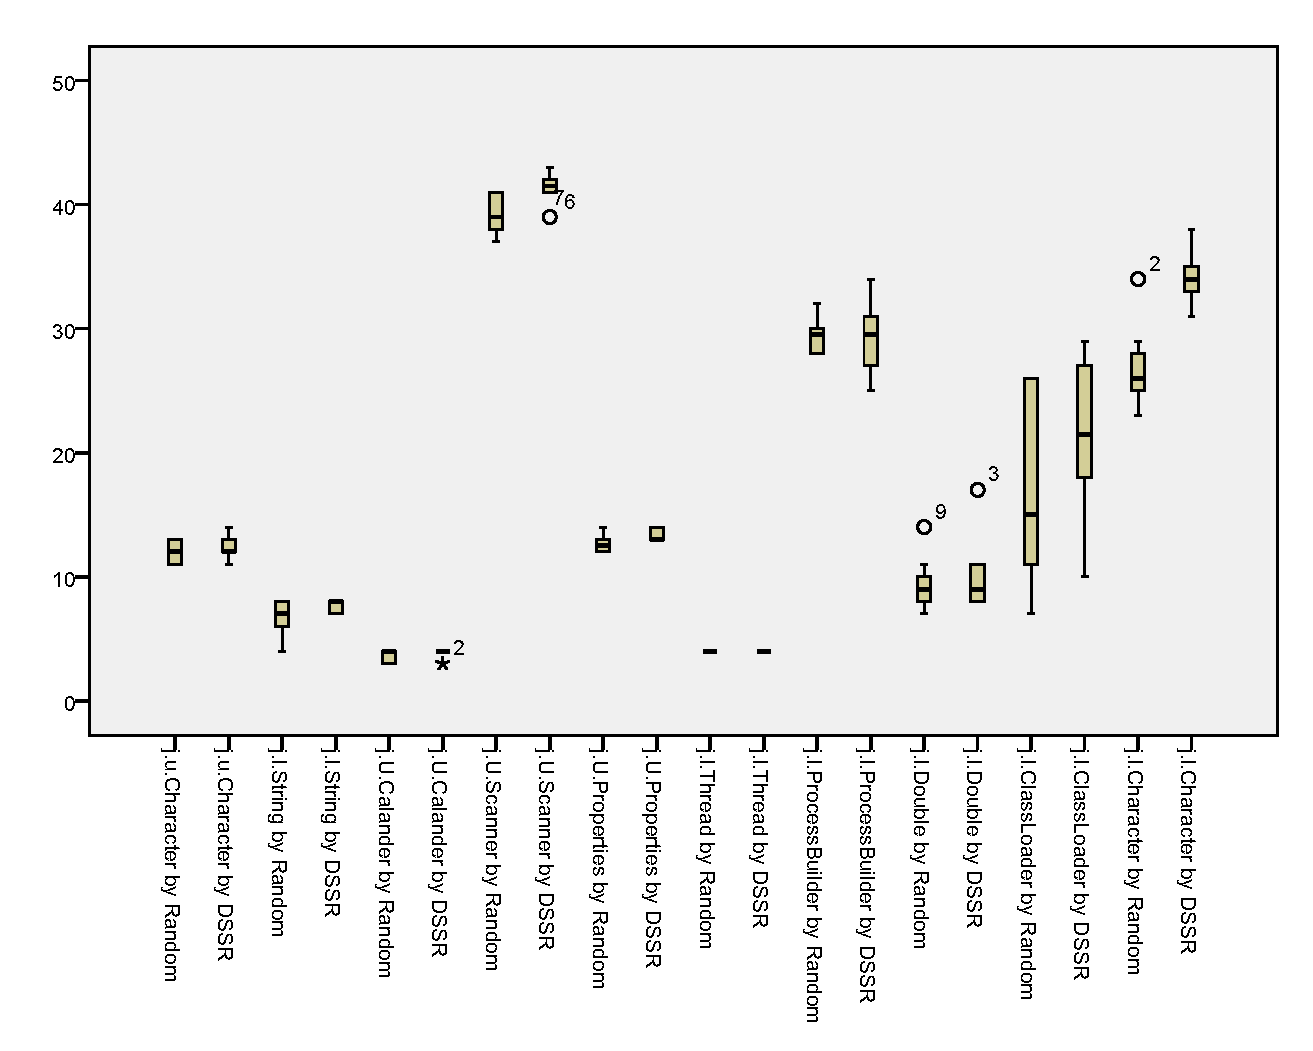
\includegraphics[width=8.5cm,height=7cm]{figures/javatests.png}
\caption{Test Results of 10 classes from java.util and java.lang package.}
\label{fig:Result2}
\end{figure}

